\section{Methods and Experimental Setup}
\label{sec:method}
\label{sec:setup}
Fig.~\ref{fig:workflow} shows the implemented workflow. Stages~1--4 construct the data and the partitions without learning any statistic; stages~5--8 use only inner-training and inner-validation groups; each outer-test fold enters only stages~9--10, after every model choice for that fold is frozen.

\begin{figure*}[t]
\centering
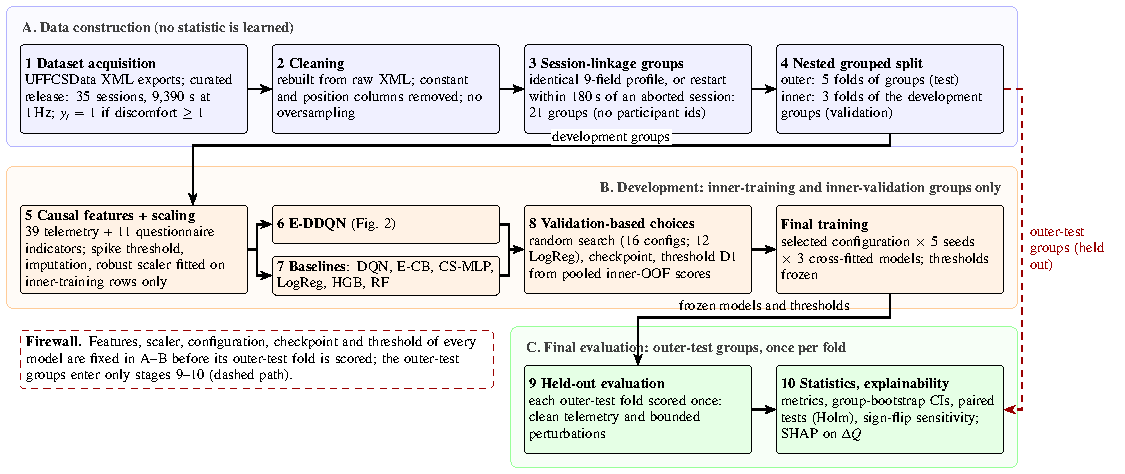
\includegraphics[width=\textwidth]{figs/v2_workflow.pdf}
\caption{Implemented workflow. A: data construction; B: development on inner folds only (E-DDQN in Fig.~\ref{fig:arch}); C: single evaluation of each outer-test fold (protocol in Fig.~\ref{fig:protocol}). The dashed path marks the outer-test groups, which bypass every fitted step.}
\label{fig:workflow}
\end{figure*}

\subsection{Data and Target (Stages 1--2)}
\label{sec:data}
UFFCSData~\cite{porcino2019uffcsdata,porcino2022identifying,porcino2021methodology} was recorded while volunteers played a race game and a flight game in a head-mounted display. About once per second the game logged speed, acceleration, three camera-rotation components (range $[-1,1]$; the parameterization is not documented), frame rate, region of interest, configuration flags and the self-reported discomfort level (0--3: none, slight, moderate, severe)~\cite{kennedy1993ssq,porcino2019demo}. Each session also stores a pre-play Cybersickness Profile Questionnaire (CSPQ: gender, age band, VR experience, glasses, vision problems, eye dominance, flicker sensitivity). We rebuilt every input from the raw XML exports: the dataset authors' curated release (\nSessionsEval{} seated sessions, December~2019; \nSamplesEval{} samples) matches \nSessionsEval{} raw exports sample by sample and is the evaluation set; the \nSessionsDev{} October-2019 standing sessions are used only to debug code and calibrate training budgets (validation cost plateaued after 20--30 epochs, so 40 epochs were fixed).

The target is $y_t=1$ (\emph{event}) if the discomfort level at second $t$ is at least~1. The prevalence is \prevEval{} (Flight \prevFlight{}, Race \prevRace{}); grades 2--3 occur in \PHGradeRaceSevere{} of \PHGradeRaceSamples{} Race but only \PHGradeFlightSevere{} of \PHGradeFlightSamples{} Flight samples. Labels are near step functions: the binary label changes \PHLabelBinaryChanges{} times per session on average, never decreases in \PHLabelNonDecreasing{} of \PHLabelSessions{} sessions, and \nEventFreeSessions{} sessions never report discomfort. The prompting procedure is not documented, so consecutive labels are a held self-report, not independent measurements. No session was attacked: $y$ marks discomfort, not a manipulation.

\subsection{Session-Linkage Groups (Stage 3)}
\label{sec:groups}
Consecutive seconds of a session are near-duplicates with the same label, so every split must keep each session---and, as far as the data allow, each participant---on one side. The release has no participant identifier, and some participants restarted after an aborted session. We link two sessions if (a)~their nine profile fields are identical or (b)~one starts within 180\,s after an aborted session ($<200$ samples) and their profiles differ in at most two fields. The connected components are \nGroupsEval{} \emph{session-linkage groups}, the unit of every split. The rule may merge different people with the same profile, which is conservative, but cannot link one person who answered the questionnaire differently in non-consecutive sessions (Section~\ref{sec:limits}).

\subsection{Causal Features and Train-Only Preprocessing (Stage 5)}
\label{sec:features}
A feature is causal if its value at second $t$ uses only seconds $0,\dots,t$ of the same session; this was verified by recomputing all features on sessions truncated at random times. The 39 telemetry features are 13 instantaneous values (game, elapsed time, speed, acceleration, $|$acceleration$|$, the three rotation components $q_t$, $\lVert q_t-q_{t-1}\rVert$, frame rate, three region-of-interest indicators), 22 trailing-window statistics over 5\,s and 15\,s (mean, SD and change of speed; mean and maximum $|$acceleration$|$; spike rate; mean and SD of rotation change; mean, minimum and drop fraction of frame rate) and 4 cumulative values (rotation change, spikes, frame drops, running mean speed). A spike is $|$acceleration$|$ above the 90th percentile of the training rows; a frame drop is a frame rate below 80\,fps. Eleven \emph{questionnaire indicators} (``profile'') encode the seven CSPQ items. The spike threshold, the imputation of the logger's zero frame rate on some first samples, and a median/IQR scaler are fitted on the training rows of each inner split and applied unchanged to its validation and test rows. Constant columns (field of view and two camera flags per game, four configuration flags, posture) and the absolute position (a proxy for elapsed course distance) are removed; no oversampling or synthetic data are used. The feature set is a hyper-parameter: \emph{telemetry} (39), \emph{telemetry+profile} (50), \emph{exposure} (8 a-priori exposure descriptors: game, elapsed time, cumulative rotation change and spikes, running and 15-s mean speed, 15-s means of rotation change and $|$acceleration$|$) or \emph{exposure+profile} (19).

\subsection{Decision Formulation: MDP or Contextual Bandit?}
\label{sec:formulation}
Each session is an episode. At second $t$ the detector observes the causal feature vector $s_t\in\mathbb{R}^d$, chooses $a_t\in\{0,1\}$ (silent, alarm) and receives $r_t=R(a_t,y_t)$ with
\begin{equation}
\begin{aligned}
R(1,1)&=+0.5, & R(0,0)&=+0.1,\\
R(0,1)&=-0.5, & R(1,0)&=-0.1.
\end{aligned}
\label{eq:reward}
\end{equation}
The next state $s_{t+1}$ is the next second of the same session; the last second is terminal ($d_t=1$). Because the telemetry was logged without an alarm in the loop, $P(s_{t+1}\mid s_t,a_t)=P(s_{t+1}\mid s_t)$, and for any $\gamma<1$
\begin{equation}
\begin{aligned}
Q^*(s,a)={}&\mathbb{E}[R(a,y_t)\mid s_t{=}s]\\
&+\underbrace{\gamma\,\mathbb{E}[(1-d_t)V^*(s_{t+1})\mid s_t{=}s]}_{\text{same for both actions}}.
\end{aligned}
\label{eq:decomp}
\end{equation}
Hence (i)~the logged-data problem is a \emph{contextual bandit}~\cite{lattimore2020bandit}: the best action maximizes the immediate expected reward for every $\gamma$. (ii)~With $p(s)=P(y=1\mid s)$ the optimal decision margin is
\begin{equation}
Q^*(s,1)-Q^*(s,0)=p(s)\,\Delta_{\mathrm{FN}}-(1-p(s))\,\Delta_{\mathrm{FP}},
\label{eq:margin}
\end{equation}
with regrets
\begin{equation}
\begin{aligned}
\Delta_{\mathrm{FN}}&=R(1,1)-R(0,1)=1.0,\\
\Delta_{\mathrm{FP}}&=R(0,0)-R(1,0)=0.2,
\end{aligned}
\label{eq:regret}
\end{equation}
so the greedy policy alarms iff $p(s)\ge\Delta_{\mathrm{FP}}/(\Delta_{\mathrm{FN}}+\Delta_{\mathrm{FP}})=1/6$: exactly the Bayes rule for costs $C_{\mathrm{FN}}:C_{\mathrm{FP}}=5:1$~\cite{elkan2001cost}. The asymmetric reward encodes an operating point, not a different objective. (iii)~Solving Eq.~\eqref{eq:margin} for $p$ maps a Q-function to a score on the nominal scale of $P(y=1\mid s)$,
\begin{equation}
\hat p(s)=\frac{\Delta Q(s)+\Delta_{\mathrm{FP}}}{\Delta_{\mathrm{FN}}+\Delta_{\mathrm{FP}}},\qquad \Delta Q(s)=Q(s,1)-Q(s,0),
\label{eq:phat}
\end{equation}
computed with each agent's own reward table ($\Delta_{\mathrm{FN}}=\Delta_{\mathrm{FP}}=2$ for the $\pm1$ reward); $\hat p$ is an uncalibrated estimate and can leave $[0,1]$. These consequences follow from known results~\cite{elkan2001cost,dudik2011efficient}; we state them because asymmetric-reward DQN detectors are usually presented without this link.

\emph{Score scale.} Class-balanced replay or minibatches (a share $1-\rho$ or one half of events instead of the training prevalence $\pi$, \SSPrevMin--\SSPrevMax) multiply the odds estimated by the scores by $k=\frac{1-\rho}{\rho}\frac{1-\pi}{\pi}$, so the nominal cut-off $\hat p\ge1/6$ corresponds to $P(y=1\mid s)\ge1/(1+5k)$: \SSEDDQNCutMin--\SSEDDQNCutMax{} for E-DDQN (approximate, since its $\gamma$ of 0.9--0.99 lets some residuals exceed the Huber threshold), \SSECBCutMin--\SSECBCutMax{} for E-CB and \SSCSMLPCutMin--\SSCSMLPCutMax{} for the balanced CS-MLP. The Huber loss with the standard DQN's $\pm1$ reward makes its $\hat p$ a nonlinear function of $P(y=1\mid s)$ (cut-off \SSDQNHuberCut{} at $\gamma=0$). These shifts affect the untuned rule D0; the primary rule D1 and the ranking metrics choose thresholds on the scores themselves, and rescaling every inner model to $P(y=1\mid s)$ changes at most \SSSensMaxChanged\,\% of D1 decisions, the cost by at most \SSSensMaxCostDelta{} and ROC-AUC by at most \SSSensMaxAucDelta{} (Supplementary Sec.~S5.12).

\emph{Episode termination and discounting.} Earlier DQN classifiers end an episode when a minority sample is misclassified~\cite{lin2020imbalanced,yang2024drlimbalanced}; a miss then also forfeits $\gamma V(s_{t+1})$, an extra $\gamma$-dependent penalty, so the problem is no longer a bandit. E-DDQN ends episodes only with the session, so Eqs.~\eqref{eq:decomp}--\eqref{eq:phat} apply. Bootstrapping ($\gamma>0$) only adds the action-independent term of Eq.~\eqref{eq:decomp} and its estimation noise; we therefore tune $\gamma\in\{0,0.5,0.9,0.99\}$ on validation data and also evaluate the separately tuned $\gamma=0$ special case (E-CB). Adaptive sequential control would require an intervention in the loop, which the data do not contain, so we make no such claim.

\subsection{E-DDQN (Stage 6)}
\label{sec:eddqn}
Fig.~\ref{fig:arch} shows E-DDQN as implemented; Table~\ref{tab:settings} lists its settings and search space. A multilayer trunk (Linear, batch or layer normalization~\cite{ioffe2015bn}, ReLU and dropout~\cite{srivastava2014dropout} except after the last layer) feeds a dueling head~\cite{wang2016dueling}, $Q(s,a)=V(s)+A(s,a)-\frac12\sum_{a'}A(s,a')$. The Double-DQN target~\cite{vanhasselt2016double} is
\begin{equation}
y_t=r_t+\gamma(1-d_t)\,Q_{\theta^-}\big(s_{t+1},\arg\max_{a'}Q_\theta(s_{t+1},a')\big),
\label{eq:ddqn}
\end{equation}
with the arg-max taken by the online network in evaluation mode ($y_t=r_t$ for $\gamma=0$). The Huber loss~\cite{huber1964robust,girshick2015fast} between $Q_\theta(s_t,a_t)$ and $y_t$ is minimized with Adam~\cite{kingma2015adam}, weight decay, gradient-norm clipping and cosine learning-rate decay~\cite{loshchilov2017sgdr}. After each update $\theta^-\leftarrow(1-\tau)\theta^-+\tau\theta$~\cite{lillicrap2016continuous}, and batch-normalization statistics are copied (all five selected E-DDQN networks used layer normalization, so this copy was inactive in the reported runs). Minibatches from the replay buffer~\cite{lin1992selfimproving} (50,000 transitions; 100,000 with full-information replay) contain a fixed share $\rho$ of non-event and $1-\rho$ of event transitions. Actions are $\varepsilon$-greedy, with an optional warm-up of random actions. With \emph{full-information replay} (tuned on/off) the action not taken is also stored with its own reward---a valid transition that the labels allow offline. Every second epoch the inner-validation groups are scored and the epoch with the lowest achievable 5:1 cost is kept (Algorithm~\ref{alg:eddqn}).

\begin{figure*}[t]
\centering
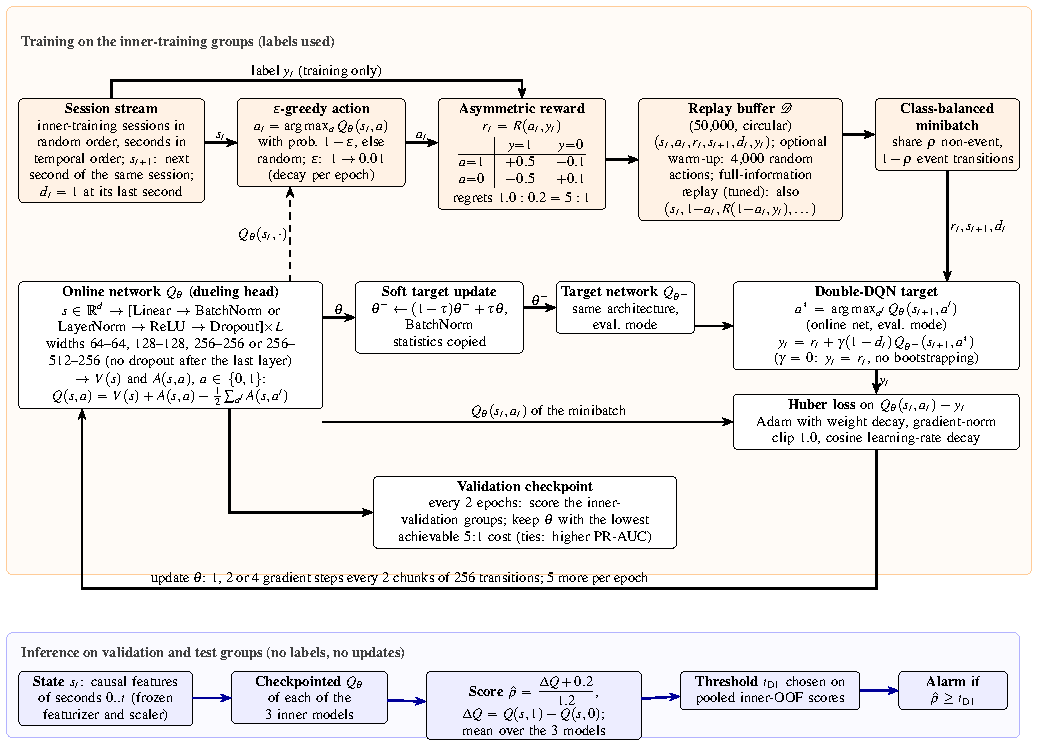
\includegraphics[width=\textwidth]{figs/v2_eddqn.pdf}
\caption{E-DDQN as implemented. Top (orange): training on the inner-training groups, where labels define the reward; bottom (blue): inference on validation and test groups with the checkpointed networks, the score of Eq.~\eqref{eq:phat} and the validation-chosen threshold of rule D1. Dashed: the online network selects actions; $\gamma=0$ removes the target-network path.}
\label{fig:arch}
\end{figure*}

\begin{algorithm}[t]
\caption{E-DDQN training for one inner split}
\label{alg:eddqn}
\begin{algorithmic}[1]
\small
\State Initialize $\theta$, $\theta^-\!\leftarrow\theta$, buffer $\mathcal{D}$; optional warm-up with random actions
\For{epoch $=1,\dots,40$}
  \State Concatenate training sessions in random order, each in temporal order; last second of each session terminal
  \For{each chunk of 256 consecutive transitions}
    \State $a_t\gets$ $\varepsilon$-greedy on $Q_\theta(s_t,\cdot)$;\ $r_t\gets R(a_t,y_t)$
    \State store $(s_t,a_t,r_t,s_{t+1},d_t,y_t)$ [and $(s_t,1-a_t,R(1-a_t,y_t),\dots)$ if full-information]
    \State every 2 chunks: 1, 2 or 4 updates on class-balanced minibatches with Eq.~\eqref{eq:ddqn}, Huber loss, Polyak update
  \EndFor
  \State 5 consolidation updates; decay $\varepsilon$; cosine LR step
  \State every 2 epochs: keep $\theta$ if the validation 5:1 cost improves
\EndFor
\State \Return checkpoint; score $\hat p(s)$ by Eq.~\eqref{eq:phat}
\end{algorithmic}
\end{algorithm}

\emph{Implementation checks.} An earlier implementation of this study built transitions from shuffled rows without terminal flags, stored the label as the action while rewarding a different action, and averaged only parameters into the target network. Unit tests guard against all three. On the real folds, every one of the \PVTransitions{} transitions written to the replay buffer in shortened runs of E-DDQN, E-CB and the standard DQN with each fold's selected configuration was logged: each stored reward is that of the stored action and the label of its state, each non-terminal next state is the next second of the same session, and terminal flags occur exactly at session ends (Supplementary Sec.~S8).

\subsection{Baselines (Stage 7)}
\label{sec:baselines}
Every baseline receives the same splits, candidate feature sets, search procedure and number of configurations (16; 12 for logistic regression), checkpoint rule (neural models), cross-fitting and threshold rules (Table~\ref{tab:settings}). The number of configurations is matched, not the coverage: the search spaces range from about \PHSpaceEDDQNMillion{} million configurations (E-DDQN) to \PHSpaceRF{} (random forest; Supplementary Sec.~S2.1). The \textbf{standard DQN}~\cite{mnih2015human} uses a symmetric $\pm1$ reward, a plain head, the max-operator target, periodic hard target copies and uniform replay; \textbf{E-CB} is E-DDQN with $\gamma=0$; the \textbf{CS-MLP} is a multilayer perceptron with event-weighted cross-entropy ($w=5$); \textbf{logistic regression}, \textbf{histogram gradient boosting (HGB)} and a \textbf{random forest (RF)}~\cite{pedregosa2011sklearn} use class weight 5. A weighted classifier estimates $p_w=5p/(5p+1-p)$, which is mapped back by
\begin{equation}
\hat p=\frac{p_w}{5-4p_w},
\label{eq:unweight}
\end{equation}
so that all models share the nominal scale of Eq.~\eqref{eq:phat}. \emph{Always alarm} and \emph{never alarm} are trivial references. Because exposure duration drives cybersickness~\cite{kennedy2000duration} and most selected configurations used exposure features, two exposure-time baselines were specified after the primary analysis and run under the same protocol: \textbf{Time-LR} (logistic regression on elapsed time) and \textbf{Time+game HGB}.

\begin{table}[t]
\centering
\caption{Implementation and training settings (\texttt{configs/protocol.json}, except the rows marked $^\dagger$; braces: searched values).}
\label{tab:settings}
\scriptsize
\setlength{\tabcolsep}{2.5pt}
\begin{tabular}{@{}p{0.27\columnwidth}p{0.70\columnwidth}@{}}
\toprule
Item & Setting \\
\midrule
Splits & outer \nOuter{} / inner \nInner{} stratified group folds (game $\times$ label); seeds 20261012 / 20261013--17 \\
Search & random, 16 configurations per family (LogReg 12 of 24), drawn once (sampling seed 777 + family index; training seed 777); objective: pooled OOF 5:1 cost at its best threshold, ties PR-AUC \\
Neural (all) & feature set \{4 sets\}; trunk \{64--64, 128--128, 256--256, 256--512--256\}; dropout \{0, .1, .2, .3\}; norm \{batch, layer\}; learning rate $\eta$ \{3e-4, 1e-3, 3e-3\}, cosine to 1e-5; weight decay \{0, 1e-4, 1e-3\}; batch \{256, 512\}; 40 epochs; checkpoint every 2 epochs \\
Agents (all) & Huber loss (threshold 1), Adam, grad.-norm clip 1.0; buffer 50,000 (100,000 with full information); chunks of 256, learning step every 2 chunks with \{1, 2, 4\} updates, 5 consolidation updates per epoch; $\varepsilon$ 1.0$\rightarrow$0.01, decay \{0.90, 0.95, 0.97\}/epoch; warm-up \{0, 4,000\} \\
E-DDQN & reward Eq.~\eqref{eq:reward}; dueling; double; soft target $\tau$ \{0.005, 0.01, 0.05\}; $\gamma$ \{0, 0.5, 0.9, 0.99\}; balanced replay $\rho$ \{0.4, 0.5, 0.6\}; full-information \{off, on\} \\
E-CB & as E-DDQN with $\gamma=0$; $\rho$, full-information searched \\
DQN & $\pm1$ reward; plain head; max target; hard copy every \{10, 100, 500\} updates; $\gamma$ \{0, 0.5, 0.9, 0.99\}; uniform replay; no full-information replay \\
CS-MLP & weighted cross-entropy ($w=5$); minibatches \{uniform, balanced\} \\
LogReg & $C$ \{1e-4, \dots, 10\} (6 values) \\
HGB & $\eta$ \{.02, .05, .1\}; iterations \{50, 100, 200, 400\}; leaves \{4, 8, 16, 31\}; min.\ leaf \{20, 100, 300\}; $\ell_2$ \{0, 1, 10\} \\
RF & 300 trees; depth \{3, 5, 8, none\}; min.\ leaf \{5, 25, 100, 300\}; features \{sqrt, 0.5, 1.0\} \\
Final & 5 seeds (1000--1004) $\times$ \nInner{} cross-fitted inner models per outer fold \\
Inference$^\dagger$ & group bootstrap, 2,000 replicates (analysis code committed with the protocol); exact sign-flip test over $2^{21}$ sign patterns (post hoc) \\
Software$^\dagger$ & Python 3.13, PyTorch~\cite{paszke2019pytorch} 2.14.1 (run on the CPU), scikit-learn 1.9.1; one thread per process; full pipeline about 2.5--3.5\,h on four CPU cores; \authorinput{CPU model and memory to be added} \\
\bottomrule
\end{tabular}
\end{table}

\subsection{Evaluation Protocol and Statistics (Stages 4 and 8--10)}
\label{sec:protocol}
\label{sec:seeds}
Fig.~\ref{fig:protocol} shows the protocol; its split, search, checkpoint, threshold and seed rules were committed before any model was trained on the evaluation sessions (the post-hoc additions are marked). The \nGroupsEval{} groups are split into \nOuter{} outer folds; each serves once as test data and the rest form its development set, which is split into \nInner{} inner folds so that every development second receives one out-of-fold (OOF) validation prediction. For each family and outer fold: (1)~each configuration is trained on the three inner splits with one seed, and the one with the lowest pooled-OOF 5:1 cost $c=(5\,\mathrm{FN}+\mathrm{FP})/N$ is selected; (2)~it is retrained with five seeds, keeping the three checkpointed inner models per seed (cross-fitting), whose mean is the test score; (3)~thresholds are chosen on the pooled OOF scores of these final models: the primary rule \emph{D1} minimizes the 5:1 cost (ties: closest to $1/6$); secondary rules are \emph{D0}, the fixed cut-off $\hat p\ge1/6$ (the greedy policy for the asymmetric agents), and an OOF recall of at least 0.95. Each OOF score comes from one inner model, whereas each test score averages three, so averaging can make test scores less spread than the scores on which the threshold was chosen; (4)~the outer-test fold is scored once, on clean and on perturbed telemetry. Checks on the real folds confirm that no session, linkage group, exact questionnaire profile, raw telemetry row or feature vector crosses a partition boundary in any of the 15 outer~$\times$~inner splits, that preprocessing is unaffected by evaluation rows, and that every configuration, checkpoint and threshold is reproduced from inner-validation data alone (Supplementary Sec.~S8). This establishes session- and linkage-group-disjoint evaluation, not participant independence.

\begin{figure*}[t]
\centering
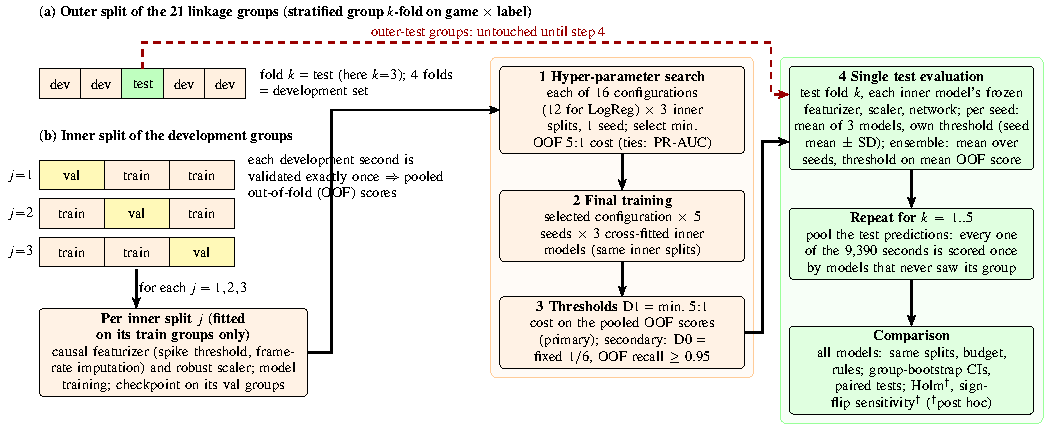
\includegraphics[width=\textwidth]{figs/v2_protocol.pdf}
\caption{Nested, session-linkage-grouped evaluation protocol, applied identically to every model. Within each outer fold, all fitting, selection, checkpointing and thresholding use inner folds of the development groups; the outer-test groups are used once, in step~4.}
\label{fig:protocol}
\end{figure*}

\emph{Seed means and seed ensemble.} We report mean~$\pm$~SD over the five seeds. Analyses that need one prediction per sample (paired tests, confidence intervals, comparison with always alarming, event-level metrics, matched operating points, perturbations, cost curves) use the \emph{seed ensemble}, the mean score over seeds thresholded on the mean OOF score; this was fixed in the evaluation code before the evaluation. The two can differ: E-DDQN's ensemble cost is \PHEnsEDDQNCost{} against a seed mean of \EDDQNCostCostMean, the standard DQN's \PHEnsDQNCost{} against \DQNCostCostMean. No seed was selected or discarded.

\emph{Metrics and inference.} We report recall, specificity, balanced accuracy, MCC~\cite{chicco2020mcc}, missed events, false positives, the 5:1 cost, ROC-AUC and PR-AUC~\cite{saito2015pr} (further metrics in Supplementary Sec.~S3.1) and event-level alarm fractions. Confidence intervals are percentile intervals of a bootstrap over the \nGroupsEval{} linkage groups (2,000 replicates); they describe the sampling of test groups given the trained models, not retraining variability beyond the five seeds. The primary paired test is a group bootstrap of the seed-ensemble cost difference, $p=2\min\{\Pr(\Delta^*\le0),\Pr(\Delta^*\ge0)\}$ (resolved to about 0.001); it was implemented in the analysis code committed with the frozen protocol and yields effect size, CI and $p$-value from one distribution. An exact group sign-flip test over all $2^{21}$ sign patterns, added after a pre-submission review, is the sensitivity analysis. Every comparison is reported as an effect size with its 95\,\% CI and Holm-adjusted~\cite{holm1979simple} $p$-values, and a difference is treated as firmly established only if it is significant under both procedures. With \nGroupsEval{} unequal groups, cluster-bootstrap inference is approximate and can be anti-conservative~\cite{cameron2008bootstrap}, so $p$-values between 0.01 and 0.05 are read as approximate. Sample-level McNemar tests~\cite{mcnemar1947,dietterich1998tests} are secondary because consecutive seconds are dependent.

\emph{Post-hoc analyses} (Supplementary Sec.~S5). The following were specified after the primary results were known and committed before being run, unless stated otherwise: the exposure-time baselines; Holm adjustment of the six comparisons with E-DDQN; comparison with always alarming (its Holm adjustment added without prior commitment); session-level bootstrap and leave-one-group-out jackknife; validation-chosen cost curves over cost ratios $R$ from 1 to 20; within-fold ROC-AUC, sign-flip tests and feature-set tallies (after review, with all results known); a \emph{search-draw experiment}, specified with three decision rules and committed before it was run, which re-tunes E-DDQN and the standard DQN with two further random draws of 16 configurations and one exposure-only draw (Supplementary Sec.~S5.11); and the descriptive score-scale calculation above (added in the final pre-submission check). The paired comparisons of the exposure-time baselines with the primary models and the Q-value-scale diagnostic were added without prior commitment.

\subsection{Telemetry-Perturbation Stress Tests and Explainability}
\label{sec:threat}
\label{sec:shap}
The motivating threats degrade frame pacing, distort camera or locomotion motion, or manipulate the field of view~\cite{odeleye2021framerate,tseng2022dark,kundu2025securing}. The data contain no attacked sessions, so we use bounded, synthetic changes of the outer-test telemetry as a stress test of which inputs the detectors use; features are recomputed with the frozen featurizer and scaler, and labels are unchanged. The 24 variants, fixed before evaluation, are frame-rate capping, orientation jitter, speed up-scaling and acceleration-spike injection at three strengths, applied to the whole session or one 60-s window (values and bounds in Supplementary Sec.~S4.1; the 60- and 45-fps caps lie below every Flight frame rate after the first second, \SSFpsFlightMin--\SSFpsFlightMax\,fps). Field-of-view manipulation is not evaluated because it never varies within a game. An adaptive adversary with label knowledge picks, per session, among 17 whole-session variants (including five ``hiding'' manipulations that mask stress signals: speed down-scaling, orientation smoothing, frame-rate restoration) the one that minimizes alarms on event seconds or maximizes alarms on non-event seconds; these are lower bounds, weaker than gradient-based attacks~\cite{kundu2025securing,ahmed2025adversarialvr}. Post hoc, SHAP values~\cite{lundberg2017shap} of the decision margin $\Delta Q$ are computed for one separately retrained E-DDQN model per outer fold with the expected-gradients estimator (DeepExplainer~\cite{shrikumar2017deeplift} failed its additivity check on the layer-normalized networks; Supplementary Sec.~S9.8).
